\documentclass[11pt,a4paper]{article}

\usepackage[utf8]{inputenc}
\usepackage[T1]{fontenc}
\usepackage[english]{babel}
\usepackage{lmodern}
\usepackage[margin=2.5cm]{geometry}
\usepackage{graphicx}
\usepackage{booktabs}
\usepackage{tabularx}
\usepackage{enumitem}
\usepackage[hidelinks]{hyperref}

\setlist{nosep}

\title{Cerio\\[0.3em]\large Project Documentation}
\author{}
\date{\today}

\begin{document}

\maketitle
\tableofcontents
\newpage

% ------------------------------------------------------------
\section{Overview}

The subject of the project is the development of a two-dimensional platform game that is
simply Super Mario (a side-scrolling Mario clone with original graphics), running in a web
browser, and, as its main part, the design, training and comparison of two approaches to
automatic level completion by a bot: neuroevolution and reinforcement learning (RL).

The game itself runs entirely on the client, in the browser. The neural networks that drive
the bot are trained and run on a server, which is written in Python.

% ------------------------------------------------------------
\section{Game rules}

The main goal of the game is to reach the flagpole at the end of the level. The game consists
of procedurally generated, side-scrolling levels. Death sends the player back to the start of
the level. Each level contains:
\begin{itemize}
  \item a level entrance and exit (flagpole),
  \item ground, platforms and blocks the player can stand on and jump between,
  \item pits and enemies capable of killing the player.
\end{itemize}
Some levels also contain items, e.g.\ question blocks with mushrooms. Completing a level
activates a checkpoint, so it does not have to be repeated.

\subsection{Game goals}

\begin{description}
  \item[Main goal:] reaching the flagpole.
  \item[Intermediate goals:] jumping over pits, avoiding or stomping enemies, collecting
        power-ups, reaching checkpoints.
  \item[Bonus goals:] collecting bonus points (coins).
  \item[Failure condition:] falling into a pit or contact with an enemy while small, which
        restarts the level.
\end{description}

\subsection{Game mechanics}

The mechanics follow the original Mario games.

\begin{itemize}
  \item running left and right, jumping (jump height depends on how long the button is held),
        crouching, attacking,
  \item stomping enemies (the set of enemy types is still being decided),
  \item pits, solid blocks, bricks, question blocks, coins,
  \item pipes that lead to bonus sub-areas and back,
  \item power-ups from Super Mario Bros.\ 1--3: Super Mushroom, Fire Flower, Super Star,
        Stopwatch, Super Leaf, Tanooki Suit, Frog Suit and Hammer Suit.
\end{itemize}

Not included: 1-Up, Heart, Bomb, Magic Potion, Magic Whistle, Goomba's Shoe and P-Wing. The game has
no P-meter, no Tanooki statue, no level timer and no swimming levels.

\textbf{Available movement actions:} move left, move right, jump, run (sprint), down
(crouch, enter pipe), attack (fireball, hammer, tail).

\subsection{Level generation}

Levels are procedurally generated from segments cut out of the original Mario levels. A
segment is a fixed-size block of tiles (16$\times$15 tiles, i.e.\ $256\times240$~px) with
tags (theme, difficulty) and left and right joints (ground height at the edge). Segments are
connected only if their joints match. The length of a level is set by the dataset (an average
Mario level is about 13 segments, $3360\times240$~px). The same seed gives the same level.

Levels are organized like a machine learning dataset: difficulty tiers (easy, medium, hard),
each split into training, validation and test levels with disjoint seeds. The 10 test levels
are frozen as files. Each level has metrics (length, gaps, enemies, difficulty score, human
time).

Mechanics from the previous draft that do not exist in Mario (dash, wall climbing, stamina,
buttons and levers) are removed from the project.

% ------------------------------------------------------------
\section{Architecture}

The game must run in a web browser, so Pygame is not used. The system has two parts.

\begin{description}
  \item[Client (browser):] a TypeScript application drawing the game on an HTML5 Canvas. It
        handles input, rendering, the fixed-timestep game loop and level loading. The client
        contains the complete, working game and can be played without the server.
  \item[Server (Python):] trains the neural networks and stores the models. It exposes the
        trained bots to the client over a WebSocket connection: the client sends the current
        observation, the server answers with the next action. The neural network backend may
        therefore live on the server, while the client only needs a working game.
\end{description}

\subsection{Game core}

The game logic is a single, deterministic simulation module without any dependency on the
rendering layer. The same code runs in the browser (with graphics) and headless on the server
side (Node.js) for training. Determinism is ensured by a fixed timestep, integer (sub-pixel)
arithmetic and a seeded random number generator. This is a necessary condition for fair
comparison of the bots and for reproducible training.

\subsection{Training environment}

Python reaches the headless core through a Gym-style interface (\texttt{reset}, \texttt{step}
returning observation, reward and done flag). Many environment instances are run in parallel
and batched to keep the training throughput high.

\begin{description}
  \item[Observation:] a tile window around the character (solid blocks, enemies, items) and
        the character state (velocity, size, power-up). No image is used.
  \item[Actions:] a small discrete set of button combinations (e.g.\ none, right,
        right+jump, right+run, right+run+jump, left, jump).
  \item[Action repeat:] a decision is made every few frames, which also keeps the
        client--server latency during live play acceptable.
\end{description}

% ------------------------------------------------------------
\section{Bot}

\subsection{Operation}

The bot reads game metadata instead of an image: the level layout, enemies, items and the
character state. Based on this data it selects the next button combination and moves towards
the flagpole. The bot completes previously unseen procedural levels.

\subsection{Approaches}

Both approaches use the same observation, action set, level generator and simulation budget,
so their results can be compared directly.

\begin{enumerate}
  \item \textbf{Neuroevolution.} A population of neural network policies is evolved with a
        genetic algorithm (or NEAT as an alternative). Fitness rewards the distance covered
        and level completion and penalizes the time used.
  \item \textbf{Reinforcement learning.} A policy trained with a policy-gradient method
        in PyTorch. The reward is based on progress to the right, a small time penalty, a
        death penalty and a bonus for reaching the flagpole.
\end{enumerate}

\subsection{Comparison of RL and neuroevolution}

The two approaches are compared on:
\begin{itemize}
  \item the share of completed levels on the test set,
  \item the completion time relative to the human time,
  \item training cost: simulation steps and wall-clock time needed to reach the
        evaluation threshold,
  \item generalization to unseen levels and variance between training runs (several seeds).
\end{itemize}

% ------------------------------------------------------------
\section{Requirements}

\subsection{Performance requirements}

\textbf{Client:} a current desktop browser (Chrome, Firefox or Edge); resolution
$854\times480$~px, maintained at 60~FPS for 80\% of the gameplay, assuming the game is
``playable''.

\textbf{Server and training:} AMD Ryzen 5 7600X (6 cores), NVIDIA GeForce RTX 3070, 48~GB RAM.

\subsection{Evaluation criteria}

\begin{itemize}
  \item The bot must complete at least 70\% of a test set consisting of 10 levels.
  \item The bot must complete the task in finite time, shorter than three times the
        human completion time.
  \item The criteria are checked for both the neuroevolution and the RL bot, and the results
        are compared.
\end{itemize}

\subsection{Technology stack}

\begin{itemize}
  \item Client: TypeScript, HTML5 Canvas (no Pygame).
  \item Headless game core for training: Node.js (the same code as in the client).
  \item Server and neural networks: Python, PyTorch, WebSocket server (e.g.\ FastAPI).
\end{itemize}

% ------------------------------------------------------------
\section{Schedule}

\begin{table}[h]
\centering
\begin{tabularx}{\textwidth}{@{}l l X@{}}
\toprule
\textbf{Date} & \textbf{Checkpoint} & \textbf{Scope} \\
\midrule
08.10.2026 & Project requirements & Requirements, game goals, bot assumptions \\
22.10.2026 & Report & Deterministic core, shared config, browser client, headless mode, level format (JSON) \\
05.11.2026 & Milestone I & Blocks, basic enemies, pipes, SMB1 power-ups, environment interface, server link, neuroevolution bot \\
19.11.2026 & Report & SMB3 power-ups, segment import, generator, datasets (train/val/test), RL training pipeline \\
03.12.2026 & Deadline & RL bot, evolution vs RL evaluation, graphics, final report \\
\bottomrule
\end{tabularx}
\caption{Project checkpoints}
\end{table}

\begin{figure}[h]
\centering
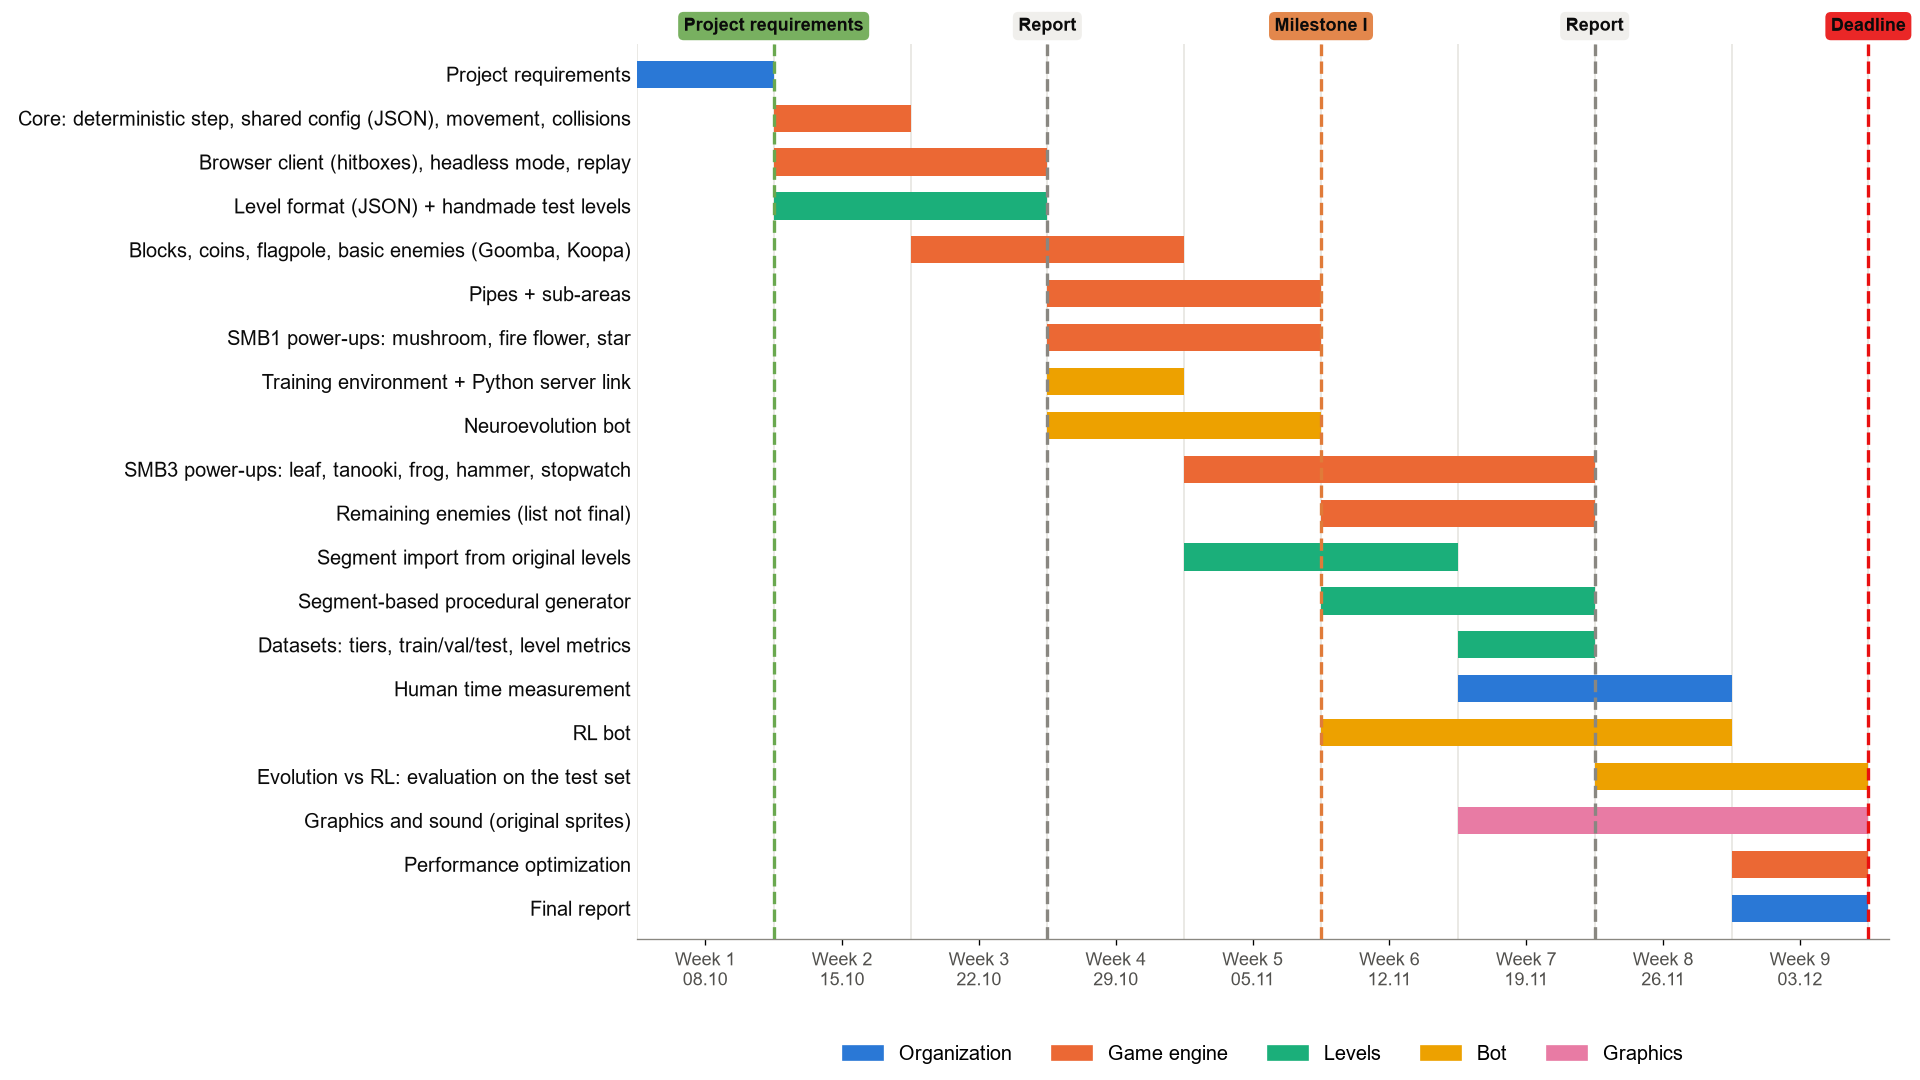
\includegraphics[width=\textwidth]{gantt-chart.png}
\caption{Gantt chart}
\end{figure}

\end{document}
